\subsubsection{Learning with Large Datasets}
\begin{itemize}[--]
	\item We want to use larger datasets because it can significantly improve our models
	\item Learning with large datasets comes with its own problems, typically computational times
	\item For example: gradient descent's update term is $\O{m}$, for each update of $\theta_j$
	\item Why not randomly choose a subset of data to train on before investing effort into creating software for large datasets
	\item If you plot can already show that $J_{cv}\approx J_{train}$ then you're already set, so there's no need to scale
\end{itemize}

\subsubsection{Stochastic Gradient Descent}
\begin{itemize}[--]
	\item Linear regression with gradient descent:
	\begin{center}
		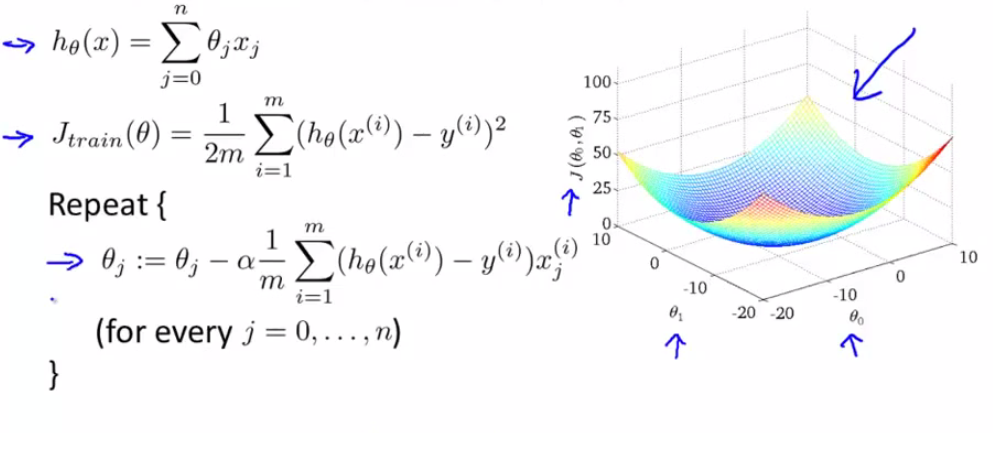
\includegraphics[scale=0.5]{sections/cs229/w14/grad_desc.png}
	\end{center}
	\item The ideas we will present are fully general, but we will use linear regression to exemplify
	\item The previous version of gradient descent we used is called \textbf{batch gradient descent}, because we're looking at a batch of examples
	\item We will redefine:
		$$cost(\theta, (x^{(i)}, y^{(i)})) = \frac{1}{2} (h(x^{i)}) - y^{(i)})^2$$
	\item We can now rewrite:
		$$J_{train}=\frac{1}{m}\sum_{i=1}^m cost(\theta, (x^{(i)}, y^{(i)}))$$
	\item Stochastic gradient descent:
	\begin{itemize}[--]
		\item Randomly suffle dataset
		\item Repeat\{ \\
			for i=1,$\ldots$,m\{ \\
				$\theta_j := \theta_j - \alpha (h(x^{(i)}) - y^{(i)})x_j^{(i)}$ for $j=0,\ldots,n$ \\
			\} \\
		\}
	\end{itemize}
	\item It's scanning through the training examples, and take a gradient descent step with the cost of just the first training example, repeating to fit a little towards each training example
	\item This outter loop allows multiple movements through the data set
	\item Batch gradient descent would make a reasonable move towards the center; however, stochastic will move more randomly as it conforms to each example
	\item It wanders around the global minimum, not necessarly finding it in the end; however, this shouldn't matter too much in most models in pratice
	\item How many times should we repeat the outer loop? 1-10x may be enough depending on the training set
\end{itemize}

\subsubsection{Mini-Batch Gradient Descent}
\begin{itemize}[--]
	\item Batch gradient descent: Use all $m$ examples in each iteration
	\item Stochastic gradient descent: USe 1 example in each iteration
	\item Mini-batch gradinet descent: Use $b$ examples in each iteration
	\item $b=$ mini-batch size (Typical range: [2, 100])
	\item This changes our update towards:
		$$\theta_j := \theta_j - \alpha\frac{1}{b}\sum_{k=i}^{i+b-1} (h(x^{(k)}) - y^{(k)} x_j^{(k)}$$
		$$i := i + b$$
	\item 
\end{itemize}

\subsubsection{Stochastic Gradient Descent Convergence}
\begin{itemize}[--]
	\item For batch gradient descent, we would plot $J_{train}$ as a function of the number of iterations, ensuring that it remained decreasing
	\item However with stochastic, you can't check the same cost function, because it uses the slow technique that it's designed to avoid
	\item Instead during learning, compute $cost(\theta, (x^{(i)}, y^{(i)}))$ before updating $\theta$ using $(x^{(i)}, y^{(i)})$
	\item Now every so many interations (say 1000) iterations, plot $cost$ averaged over the last 1000 examples processed by the algorithm
	\item These plots may be noisy
	\item As you increase the number of iterations you average, you may be able to achieve a smoother curve, but you get very little feedback
	\item Somtiems the cost won't decrease, but when increasing the iterations you may get more intution that is hidden by the noise
	\item If the curve diverges, use a smaller learning rate $\alpha$
	\item Learning rate $\alpha$ is typically held constant. It can slowly decrease over time if we want $\theta$ to converge
	\item This may not be worthwhile since you have to tune more paramteres
\end{itemize}

\subsubsection{Online Learning}
\begin{itemize}[--]
	\item If you have a continuous stream of data is use an online learning algorithm to use the prefences from the stream of data to optimize some of the decisions on the site
	\item Considering a shipping service webstie where user comes, specifies origin and destination, you offer to ship their package for some asking price, and users sometimes choose to use your shipping services ($y=1$), and sometimes not ($y=0$)
	\item Features $x$ capture properties of user, of origin/destination and asking price. We want to learn $p(y=1|x;\theta)$ to optimize price
	\item Repeat forever \{
	Get $(x,y)$ corresponding to user.
	Update $\theta$ using just the new example $(x,y)$:
		$\theta_j := \theta_j - \alpha (h(x) - y)x_j$ for $j=0,\ldots, n$
	\}
	\item We are discarding the notion of a fix training set, so no longer using ${(i)}$ notation
	\item This algorithm can adapt to changing user preferences
	\item Another example: Product search (learning to search)
	\begin{itemize}[--]
		\item User searches for ``android phone 1080p camera''
		\item Have 100 phones in store. Will return 10 results.
		\item $x=$ features of phone, how many words in user query match name of phne, how many words in query match description of phone, etc.
		\item $y=1$ if user clicks on link. $y=0$ otherwise
		\item Learn $p(y=1|x;\theta)$
		\item Learning the CTR (click-through-rate)
		\item Use to show user the 10 phones they're most likely to click on
	\end{itemize}
	\item Other examples: choosing special offers to show user; customized selection of news articles; product recommendations $\ldots$
\end{itemize}

\subsubsection{Map Reduce and Data Parallelism}
\begin{itemize}[--]
	\item We will split the training set into different subsets, and process each portion on a different computer
	\item After each machine as computed a temporary new $\theta_j$ and combine them 
		$$\theta_j := \theta_j - \alpha \frac{1}{m} (temp_j^{(1)}+\ldots+temp_j^{(\ldots)} \text{ for } j = 0,\ldots, n$$
	\item Many learning algorithms can be expressed as computing sums of functiosn over the training set
	\item You can also use this on multi-core machines
	\item Some linear algebra libraries already do multi-core computations
\end{itemize}